%%%%%%%%%%%%%%%%%%%%%%%%%%%%%%%%%%%%%%%%%%%%%%%%%%%%%%%%%%%% 
% Name: XeTeX+xeCJK日常使用模板
% Author: Lox Freeman
% Email: xiaohanyu1988@gmail.com
% 、
% 本文档可以自由转载、修改,希望能给广大TeXer的中文之路提供一些方便。
%%%%%%%%%%%%%%%%%%%%%%%%%%%%%%%%%%%%%%%%%%%%%%%%%%%%%%%%%%%% 

\documentclass[a4paper, 12pt, titlepage]{article}

%%%%%%%%%%%%%%%%%%%%%%%%% xeCJK相关宏包%%%%%%%%%%%%%%%%%%%%%%%%%
\usepackage{xltxtra,fontspec,xunicode}
\usepackage[slantfont, boldfont, CJKchecksingle]{xeCJK}

\CJKsetecglue{\hskip 0.15em plus 0.05em minus 0.05em}
% slanfont: 允许斜体
% boldfont: 允许粗体
% CJKnormalspaces: 仅忽略汉字之间的空白,但保留中英文之间的空白。
% CJKchecksingle: 避免单个汉字单独占一行。
% CJKaddspaces: [备选]忽略汉字之间的空白,并且自动在中英文转换时插入空白。

% \CJKlanguage{zh-cn}                 % 中文标点特殊处理
\XeTeXlinebreaklocale "zh"           % 针对中文进行断行
\XeTeXlinebreakskip = 0pt plus 1pt minus 0.1pt
% 给予TeX断行一定自由度
%%%%%%%%%%%%%%%%%%%%%%%%% xeCJK%%%%%%%%%%%%%%%%%%%%%%%%%%%%%%%%

%%%%%%%%%%%%% 日常所用宏包、通通放在一起%%%%%%%%%%%%%%%%%%%%%%%%%%%%
% 什么常用的宏包都可以放这里。下面是我常用的宏包,每个都给出了简要注释
\usepackage[top=2.5cm, bottom=3cm, left=2.5cm, right=2.5cm]{geometry} % 控制页边距
\usepackage{enumerate}               % 控制项目列表
\usepackage{multicol}                % 多栏显示

\usepackage[%
pdfstartview=FitH,%
CJKbookmarks=true,%
bookmarks=true,%
bookmarksnumbered=true,%
bookmarksopen=true,%
colorlinks=true,%
citecolor=seco,%
linkcolor=seco,%
anchorcolor=seco,%
urlcolor=seco%
]{hyperref}                          % 超链接相关设置

\usepackage{titlesec}                % 控制标题
\usepackage{titletoc}                % 控制目录
\usepackage{type1cm}                 % 控制字体大小
\usepackage{indentfirst}             % 首行缩进,用\noindent取消某段缩进
\usepackage{bbding}                  % 一些特殊符号
\usepackage{cite}                    % 支持引用
\usepackage{framed,color,xcolor}     % 支持彩色文本、底色、文本框等
\usepackage{latexsym}                % LaTeX一些特殊符号宏包
\usepackage{amsmath}                 % AMS LaTeX宏包
\usepackage{bm}                      % 数学公式中的黑斜体
\usepackage{relsize}                 % 调整公式字体大小:\mathsmaller, \mathlarger
\usepackage{soul}                    % 下划线自动回车换行
\usepackage{attachfile}              % 添加附见使用的宏包
\usepackage{parcolumns}              % 列排版
% \usepackage{setspace}

\makeindex                           % 生成索引

\makeatletter
\let\std@footnotetext\@footnotetext
\usepackage{setspace}
\let\@footnotetext\std@footnotetext
\makeatother

%%%%%%%%%%%%%%%%%%%%%%%%% 绘图方法%%%%%%%%%%%%%%%%%%%%%%%%%%%
\usepackage{graphicx}                % 图形宏包
\graphicspath{{./figure/}{./figures/}{./image/}{./graphics/}{./graphic/}{./pictures/}{./picture/}}

\usepackage{tikz}
\usepackage{amsmath,bm,times}
\usepackage{verbatim}

\usepackage{tabularx}

\usetikzlibrary{shapes,arrows,shadows,fit,snakes,positioning,decorations}
\usetikzlibrary{decorations.shapes}
\usetikzlibrary{calc}           %coordinate

\usepackage{caption}
\usepackage{float}

\ifx\du\undefined
\newlength{\du}
\fi
\setlength{\du}{15\unitlength}

\newlength\Textwd
\setlength\Textwd{3cm}
\newcommand\Textbox[2]{%
  \parbox[c][#1][c]{\Textwd}{\linespread{0.5}\centering#2}}

\makeatletter
\DeclareRobustCommand{\rvdots}{%
  \vbox{
    \baselineskip6\p@\lineskiplimit\z@
    \kern-\p@
    \hbox{.}\hbox{.}\hbox{.}
  }}
\makeatother

\makeatletter
\newcommand{\gettikzxy}[3]{%
  \tikz@scan@one@point\pgfutil@firstofone#1\relax
  \edef#2{\the\pgf@x}%
  \edef#3{\the\pgf@y}%
}
\makeatother
%%%%%%%%%%%%%%%%%%%%%%%%% 绘图方法结束%%%%%%%%%%%%%%%%%%%%%%%%%%%

%%%%%%%%%%%%%%%%%%%%%%%%% fancyhdr设置页眉页脚%%%%%%%%%%%%%%%%%%%%
\usepackage{etoolbox}
\usepackage{fancyhdr}                % 页眉页脚
\pagestyle{fancy}                    % 页眉页脚风格
\setlength{\headheight}{15pt}        % 有时会出现\headheight too small的warning

\makeatletter
\patchcmd{\@fancyhead}{\rlap}{\color{seco}\rlap}{}{}
\patchcmd{\headrule}{\hrule}{\color{seco}\hrule}{}{}
\patchcmd{\@fancyfoot}{\rlap}{\color{seco}\rlap}{}{}
\patchcmd{\footrule}{\hrule}{\color{seco}\hrule}{}{}
\makeatother
%%%%%%%%%%%%%%%%%%%%%%%%% fancyhdr设置结束%%%%%%%%%%%%%%%%%%%%%%%

%%%%%%%%%%%%%%%%%%%%%%%%% xeCJK字体设置%%%%%%%%%%%%%%%%%%%%%%%%%
\setmainfont[Ligatures=TeX]{Minion Pro} % (\textrm)
\setsansfont{Myriad Pro}                % (\textsf)
\setmonofont{Adobe Garamond Pro}        % Palatino Linotype

\setCJKmainfont[BoldFont={方正兰亭纤黑_GBK},ItalicFont={Adobe Kaiti Std}]{Adobe Kaiti Std}
\setCJKsansfont[BoldFont={方正兰亭纤黑_GBK}]{方正兰亭纤黑_GBK}
\setCJKmonofont{方正兰亭纤黑_GBK}
%%%%%%%%%%%%%%%%%%%%%%%%% xeCJK字体设置结束%%%%%%%%%%%%%%%%%%%%%%

%%%%%%%%%%%%%%%%%%%%%%%%% listings宏包粘贴源码%%%%%%%%%%%%%%%%%%%%
\usepackage{listings}                % 方便粘贴源代码,部分代码高亮功能
\lstloadlanguages{}                  % 所要粘贴代码的编程语言

\newfontfamily\listingsfont{Calibri}
\newfontfamily\listingsfontinline{Calibri}

\definecolor{sh_keyword}{rgb}{0.06, 0.10, 0.98}   % #101AF9
\definecolor{shadecolor}{rgb}{0.83, 0.83, 0.83}
\definecolor{monokai-grey-dark}{RGB}{39, 40, 34}   % #272822
\definecolor{monokai-yellow-light}{RGB}{248, 248, 246}   % #F8F8F2
\definecolor{monokai-green}{RGB}{166, 226, 42}
\definecolor{dark green}{rgb}{0.000000,0.392157,0.000000}
\definecolor{forest green}{rgb}{0.133333,0.545098,0.133333}
\def\lstsmallmath{\leavevmode\ifmmode \scriptstyle \else  \fi}
\def\lstsmallmathend{\leavevmode\ifmmode  \else  \fi}

% \definecolor{seco}{RGB}{9,80,3}
% \definecolor{seco}{RGB}{0,145,215}
\definecolor{seco}{RGB}{0,175,152}
\definecolor{main}{RGB}{127,191,51}

% \makeatletter
%   \newcommand\listingfont{\@setfontsize\listingfont{11pt}{13.2pt}}
% \makeatother

\renewcommand{\lstlistingname}{代码}

\lstset {
  language=c++,
  backgroundcolor=\color{monokai-grey-dark},
  % frame=shadowbox,
  % breaklines,
  % rulesepcolor=\color{red!20!green!20!blue!20},
  showspaces=false,showtabs=false,tabsize=4,
  numberstyle=\tiny\color{black},numbers=left,
  % basicstyle= \listingfont\listingsfont\color{monokai-yellow-light},
  basicstyle= \small\listingsfont\color{monokai-yellow-light},
  stringstyle=\color{dark green},
  keywordstyle = \color{monokai-green}\bfseries,
  commentstyle=\footnotesize\color{forest green}\itshape,
  captionpos=b,
  showspaces=false,showtabs=false, showstringspaces=false,
  xleftmargin=0.7cm, xrightmargin=0.5cm,
  % lineskip=-0.3em,
  breaklines=tr,
  escapebegin={\lstsmallmath}, escapeend={\lstsmallmathend},
  extendedchars=false
}

\lstnewenvironment{acol}[1][]{\lstset{language={[x86masm]Assembler},#1}}{}
\newenvironment{parcolumenv}[1] {\begin{spacing}{#1}}{\end{spacing}}
%%%%%%%%%%%%%%%%%%%%%%%%% listings宏包设置结束%%%%%%%%%%%%%%%%%%%%


%%%%%%%%%%%%%%%%%%%%%%%%% 一些关于中文文档的重定义%%%%%%%%%%%%%%%%%

%%%% 数学公式定理的重定义%%%%
\newtheorem{example}{例}                                   % 整体编号
\newtheorem{algorithm}{算法}
\newtheorem{theorem}{定理}[section]                        % 按 section 编号
\newtheorem{definition}{定义}
\newtheorem{axiom}{公理}
\newtheorem{property}{性质}
\newtheorem{proposition}{命题}
\newtheorem{lemma}{引理}
\newtheorem{corollary}{推论}
\newtheorem{remark}{注解}
\newtheorem{condition}{条件}
\newtheorem{conclusion}{结论}
\newtheorem{assumption}{假设}

%%%% 章节等名称重定义%%%%
\renewcommand{\contentsname}{目\hspace{2em}录}
\renewcommand{\indexname}{索引}
\renewcommand{\listfigurename}{插图目录}
\renewcommand{\listtablename}{表格目录}
\renewcommand{\figurename}{图}
\renewcommand{\tablename}{表}
\renewcommand{\appendixname}{附\hspace{2em}录}

%%%% 设置chapter、section与subsection的格式%%%%
\titleformat{\chapter}{\centering\huge}{\color{seco}第\thechapter{}章}{1em}{\color{seco}\textbf}
\titleformat{\section}{\centering\LARGE}{\color{seco}\thesection}{1em}{\color{seco}\textbf}
\titleformat{\subsection}{\Large}{\color{seco}\thesubsection}{1em}{\color{seco}\textbf}
%%%%%%%%%%%%%%%%%%%%%%%%% 中文重定义结束%%%%%%%%%%%%%%%%%%%%


%%%%%%%%%%%%%%%%%%%%%%%%% 一些个性设置%%%%%%%%%%%%%%%%%%%%%%
\setlength{\parskip}{0.5\baselineskip}     % 设定段间距
\linespread{1.6}                           % 设定行距
\newcommand{\pozhehao}{\kern0.3ex\rule[0.8ex]{2em}{0.1ex}\kern0.3ex}% 中文破折号,据说来自清华模板

\setCJKfamilyfont{title}{方正正中黑简体}

\newcommand*{\TitleFont}{\usefont{\encodingdefault}{\rmdefault}{b}{n}\fontsize{32}{40}\selectfont\CJKfamily{title}\color{seco}}% 标题字体设置

\renewcommand{\today}{\color{seco}\number\year 年 \number\month 月 \number\day 日}
%%%%%%%%%%%%%%%%%%%%%%%%% 个性设置结束%%%%%%%%%%%%%%%%%%%%%%


%%%%%%%%%%%%%%%%%%%%%%%%% 正文部分%%%%%%%%%%%%%%%%%%%%%%%%%
\begin{document}
\setlength{\parindent}{2em}
% 设定首行缩进为2em。注意此设置一定要在document环境之中。
% 这可能与\setlength作用范围相关

\title{\TitleFont 数据结构之排序\vspace{8cm}}
\author{\href{mailto:q00148943@gmail.com}{\LARGE{秦新良}}}
\date{\vspace{0.5cm}\today}

\maketitle

\tableofcontents
\newpage


\section{排序}
本篇介绍常用的排序算法并给出其实现,最后对各种排序算法作比较。代码\ref{lst1}给出了排序算法链表实现的链表定义。
\begin{spacing}{1.0}
  \lstinputlisting[label=lst1,caption=链表]{list/list.h}
\end{spacing}

\subsection{插入排序}
\label{subsec:labelsub1}
插入排序的一个非常形象的说明就是打牌。起牌的过程中,每次我们摸起一张牌后,都会和手中已有的牌做比较,然后将牌插到相应的位置,如图\ref{fig00}所示。
\begin{figure}[H]
  \setlength{\abovecaptionskip}{0pt}
  \centering
  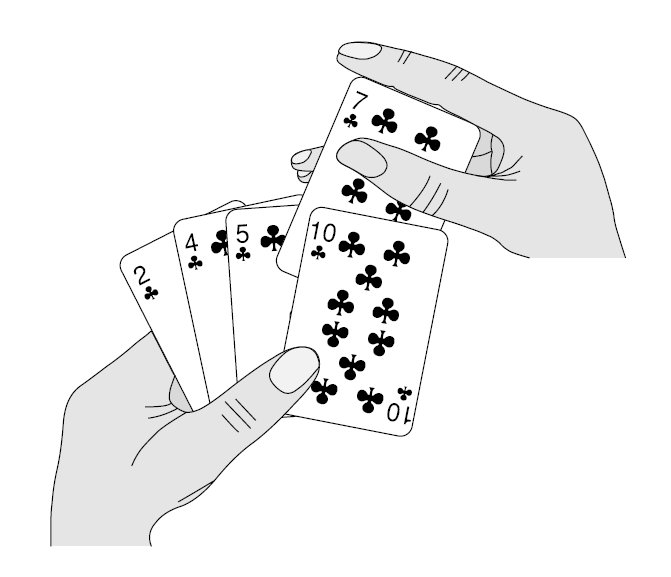
\includegraphics[width=0.6\textwidth]{playing_cards.jpg}
  \caption{打牌}
  \label{fig00}
\end{figure}


整个起牌的过程,就是对手中的牌的一次插入排序过程。当然,也不排除有的人对手中的牌并不排序,因为这样可以有效的防止“邻居偷窥“,该场景就不在我们的举例范围之内了。

插入排序的时间复杂度为O(${n}^{2}$),排序过程中只需O(1)个元素的额外空间即可完成整个数组的排序。代码\ref{lst2}给出了插入排序的C代码实现。
\begin{spacing}{1.0}
  \lstinputlisting[label=lst2,caption=插入排序]{list/insert_sort.c}
\end{spacing}


为了更清楚的理解该算法,下面以排序6、5、3、2、8、7、1、4这一组数为例来说明插入排序的算法原理。

\captionsetup[figure]{labelformat=empty}

i = 0\footnote{真实的排序不会从i = 0开始,这里用(i = 0)\&\&(j = 0)表示初始未排序。}时:
\begin{figure}[H]
  \setlength{\abovecaptionskip}{0pt}
  \definecolor{sorted}{RGB}{239,126,30}
  \definecolor{unsorted}{RGB}{0,175,152}
  \definecolor{sorting}{RGB}{127,191,51}
  \begin{center}
    \begin{tikzpicture}
      \tikzset{
        BLOCK/.style={
          draw,
          align=center,
          text height=0.2cm,
          text width=0.4cm,
          draw=black,
          rectangle split part fill={unsorted,unsorted,unsorted,unsorted,unsorted,unsorted,unsorted,unsorted},
          rectangle split, 
          rectangle split horizontal,
          rectangle split parts=#1, 
        }
      }

      \node (unsorted) [BLOCK=8]{
        \nodepart{one}\raisebox{-3.50pt}{\scriptsize 6} \strut\nodepart{two}\scriptsize 5\strut
        \nodepart{three}\scriptsize 3 \strut\nodepart{four}\scriptsize 2\strut
        \nodepart{five}\scriptsize 8 \strut\nodepart{six}\scriptsize 7\strut
        \nodepart{seven}\scriptsize 1 \strut\nodepart{eight}\scriptsize 4\strut};

      \node[xshift=-0.3cm,anchor=east] at (unsorted.west) {\scriptsize $j = 0$};
    \end{tikzpicture}
  \end{center}
  \caption{}
  \label{fig0}
\end{figure}


i = 1时:
\begin{figure}[H]
  \setlength{\abovecaptionskip}{0pt}
  \definecolor{sorted}{RGB}{239,126,30}
  \definecolor{unsorted}{RGB}{0,175,152}
  \definecolor{sorting}{RGB}{127,191,51}
  \begin{center}
    \begin{tikzpicture}
      \tikzset{
        BLOCK/.style={
          draw,
          align=center,
          text height=0.2cm,
          text width=0.4cm,
          draw=black,
          rectangle split part fill={unsorted,unsorted,unsorted,unsorted,unsorted,unsorted,unsorted,unsorted},
          rectangle split, 
          rectangle split horizontal,
          rectangle split parts=#1, 
        }
      }

      \node (node1)[BLOCK=8, rectangle split part fill={sorted,sorted,unsorted,unsorted,unsorted,unsorted,unsorted,unsorted}]{
        \nodepart{one}\raisebox{-3.5pt}{\scriptsize 5} \strut\nodepart{two}\scriptsize 6\strut
        \nodepart{three}\scriptsize 3 \strut\nodepart{four}\scriptsize 2\strut
        \nodepart{five}\scriptsize 8 \strut\nodepart{six}\scriptsize 7\strut
        \nodepart{seven}\scriptsize 1 \strut\nodepart{eight}\scriptsize 4\strut};

      \node[xshift=-0.3cm,anchor=east] at (node1.west) {\scriptsize $j = 1$};
      \draw [black, -stealth] (node1.two south) to [bend left=45] (node1.one south);
    \end{tikzpicture}
  \end{center}
  \caption{}
  \label{fig1}
\end{figure}


i = 2时:
\begin{figure}[H]
  \setlength{\abovecaptionskip}{0pt}
  \definecolor{sorted}{RGB}{239,126,30}
  \definecolor{unsorted}{RGB}{0,175,152}
  \definecolor{sorting}{RGB}{127,191,51}
  \begin{center}
    \begin{tikzpicture}
      \tikzset{
        BLOCK/.style={
          draw,
          align=center,
          text height=0.2cm,
          text width=0.4cm,
          draw=black,
          rectangle split part fill={unsorted,unsorted,unsorted,unsorted,unsorted,unsorted,unsorted,unsorted},
          rectangle split, 
          rectangle split horizontal,
          rectangle split parts=#1, 
        }
      }

      \node (node2)[BLOCK=8, rectangle split part fill={sorted,sorting,sorting,unsorted,unsorted,unsorted,unsorted,unsorted}]{
        \nodepart{one}\raisebox{-3.5pt}{\scriptsize 5} \strut\nodepart{two}\scriptsize 3\strut
        \nodepart{three}\scriptsize 6 \strut\nodepart{four}\scriptsize 2\strut
        \nodepart{five}\scriptsize 8 \strut\nodepart{six}\scriptsize 7\strut
        \nodepart{seven}\scriptsize 1 \strut\nodepart{eight}\scriptsize 4\strut};

      \node[xshift=-0.3cm,anchor=east] at (node2.west) {\scriptsize $j = 2$};
      \draw [black, -stealth] (node2.three south) to [bend left=45] (node2.two south);

      \node (node3)[BLOCK=8, right=1.8 of node2, rectangle split part fill={sorted,sorted,sorted,unsorted,unsorted,unsorted,unsorted,unsorted}]{
        \nodepart{one}\raisebox{-3.5pt}{\scriptsize 3} \strut\nodepart{two}\scriptsize 5\strut
        \nodepart{three}\scriptsize 6 \strut\nodepart{four}\scriptsize 2\strut
        \nodepart{five}\scriptsize 8 \strut\nodepart{six}\scriptsize 7\strut
        \nodepart{seven}\scriptsize 1 \strut\nodepart{eight}\scriptsize 4\strut};

      \node[xshift=-0.3cm,anchor=east] at (node3.west) {\scriptsize $j = 1$};
      \draw [black, -stealth] (node3.two south) to [bend left=45] (node3.one south);

    \end{tikzpicture}
  \end{center}
  \caption{}
  \label{fig2}
\end{figure}


i = 3时:
\begin{figure}[H]
  \setlength{\abovecaptionskip}{0pt}
  \definecolor{sorted}{RGB}{239,126,30}
  \definecolor{unsorted}{RGB}{0,175,152}
  \definecolor{sorting}{RGB}{127,191,51}
  \begin{center}
    \begin{tikzpicture}
      \tikzset{
        BLOCK/.style={
          draw,
          align=center,
          text height=0.2cm,
          text width=0.4cm,
          draw=black,
          rectangle split part fill={unsorted,unsorted,unsorted,unsorted,unsorted,unsorted,unsorted,unsorted},
          rectangle split, 
          rectangle split horizontal,
          rectangle split parts=#1, 
        }
      }

      \node (node4)[BLOCK=8, rectangle split part fill={sorted,sorted,sorting,sorting,unsorted,unsorted,unsorted,unsorted}]{
        \nodepart{one}\raisebox{-3.5pt}{\scriptsize 3} \strut\nodepart{two}\scriptsize 5\strut
        \nodepart{three}\scriptsize 2 \strut\nodepart{four}\scriptsize 6\strut
        \nodepart{five}\scriptsize 8 \strut\nodepart{six}\scriptsize 7\strut
        \nodepart{seven}\scriptsize 1 \strut\nodepart{eight}\scriptsize 4\strut};

      \node[xshift=-0.3cm,anchor=east] at (node4.west) {\scriptsize $j = 3$};
      \draw [black, -stealth] (node4.four south) to [bend left=45] (node4.three south);

      \node (node5)[BLOCK=8, right=1.8 of node4, rectangle split part fill={sorted,sorting,sorting,sorted,unsorted,unsorted,unsorted,unsorted}]{
        \nodepart{one}\raisebox{-3.5pt}{\scriptsize 3} \strut\nodepart{two}\scriptsize 2\strut
        \nodepart{three}\scriptsize 5 \strut\nodepart{four}\scriptsize 6\strut
        \nodepart{five}\scriptsize 8 \strut\nodepart{six}\scriptsize 7\strut
        \nodepart{seven}\scriptsize 1 \strut\nodepart{eight}\scriptsize 4\strut};

      \node[xshift=-0.3cm,anchor=east] at (node5.west) {\scriptsize $j = 2$};
      \draw [black, -stealth] (node5.three south) to [bend left=45] (node5.two south);

      \node (node6)[BLOCK=8, below=1 of node4, rectangle split part fill={sorted,sorted,sorted,sorted,unsorted,unsorted,unsorted,unsorted}]{
        \nodepart{one}\raisebox{-3.5pt}{\scriptsize 2} \strut\nodepart{two}\scriptsize 3\strut
        \nodepart{three}\scriptsize 5 \strut\nodepart{four}\scriptsize 6\strut
        \nodepart{five}\scriptsize 8 \strut\nodepart{six}\scriptsize 7\strut
        \nodepart{seven}\scriptsize 1 \strut\nodepart{eight}\scriptsize 4\strut};

      \node[xshift=-0.3cm,anchor=east] at (node6.west) {\scriptsize $j = 1$};
      \draw [black, -stealth] (node6.two south) to [bend left=45] (node6.one south);

    \end{tikzpicture}
  \end{center}
  \caption{}
  \label{fig3}
\end{figure}


i = 4时:
\begin{figure}[H]
  \setlength{\abovecaptionskip}{0pt}
  \definecolor{sorted}{RGB}{239,126,30}
  \definecolor{unsorted}{RGB}{0,175,152}
  \definecolor{sorting}{RGB}{127,191,51}
  \begin{center}
    \begin{tikzpicture}
      \tikzset{
        BLOCK/.style={
          draw,
          align=center,
          text height=0.2cm,
          text width=0.4cm,
          draw=black,
          rectangle split part fill={unsorted,unsorted,unsorted,unsorted,unsorted,unsorted,unsorted,unsorted},
          rectangle split, 
          rectangle split horizontal,
          rectangle split parts=#1, 
        }
      }

      \node (node7)[BLOCK=8, rectangle split part fill={sorted,sorted,sorted,sorted,sorted,unsorted,unsorted,unsorted}]{
        \nodepart{one}\raisebox{-3.5pt}{\scriptsize2} \strut\nodepart{two}\scriptsize3\strut
        \nodepart{three}\scriptsize 5 \strut\nodepart{four}\scriptsize 6\strut
        \nodepart{five}\scriptsize 8 \strut\nodepart{six}\scriptsize 7\strut
        \nodepart{seven}\scriptsize 1 \strut\nodepart{eight}\scriptsize 4\strut};

      \node[xshift=-0.3cm,anchor=east] at (node7.west) {\scriptsize $j = 4$};
    \end{tikzpicture}
  \end{center}
  \caption{}
  \label{fig4}
\end{figure}


i = 5时:
\begin{figure}[H]
  \setlength{\abovecaptionskip}{0pt}
  \definecolor{sorted}{RGB}{239,126,30}
  \definecolor{unsorted}{RGB}{0,175,152}
  \definecolor{sorting}{RGB}{127,191,51}
  \begin{center}
    \begin{tikzpicture}
      \tikzset{
        BLOCK/.style={
          draw,
          align=center,
          text height=0.2cm,
          text width=0.4cm,
          draw=black,
          rectangle split part fill={unsorted,unsorted,unsorted,unsorted,unsorted,unsorted,unsorted,unsorted},
          rectangle split, 
          rectangle split horizontal,
          rectangle split parts=#1, 
        }
      }

      \node (node7)[BLOCK=8, rectangle split part fill={sorted,sorted,sorted,sorted,sorted,sorted,unsorted,unsorted}]{
        \nodepart{one}\raisebox{-3.5pt}{\scriptsize 2} \strut\nodepart{two}\scriptsize 3\strut
        \nodepart{three}\scriptsize 5 \strut\nodepart{four}\scriptsize 6\strut
        \nodepart{five}\scriptsize 7 \strut\nodepart{six}\scriptsize 8\strut
        \nodepart{seven}\scriptsize 1 \strut\nodepart{eight}\scriptsize 4\strut};

      \node[xshift=-0.3cm,anchor=east] at (node7.west) {\scriptsize $j = 5$};
      \draw [black, -stealth] (node7.six south) to [bend left=45] (node7.five south);

    \end{tikzpicture}
  \end{center}
  \caption{}
  \label{fig5}
\end{figure}


i = 6时:
\begin{figure}[H]
  \setlength{\abovecaptionskip}{0pt}
  \definecolor{sorted}{RGB}{239,126,30}
  \definecolor{unsorted}{RGB}{0,175,152}
  \definecolor{sorting}{RGB}{127,191,51}
  \begin{center}
    \begin{tikzpicture}
      \tikzset{
        BLOCK/.style={
          draw,
          align=center,
          text height=0.2cm,
          text width=0.4cm,
          draw=black,
          rectangle split part fill={unsorted,unsorted,unsorted,unsorted,unsorted,unsorted,unsorted,unsorted},
          rectangle split, 
          rectangle split horizontal,
          rectangle split parts=#1, 
        }
      }

      \node (node7)[BLOCK=8, rectangle split part fill={sorted,sorted,sorted,sorted,sorted,sorting,sorting,unsorted}]{
        \nodepart{one}\raisebox{-3.5pt}{\scriptsize 2} \strut\nodepart{two}\scriptsize 3\strut
        \nodepart{three}\scriptsize 5 \strut\nodepart{four}\scriptsize 6\strut
        \nodepart{five}\scriptsize 7 \strut\nodepart{six}\scriptsize 1\strut
        \nodepart{seven}\scriptsize 8 \strut\nodepart{eight}\scriptsize 4\strut};

      \node[xshift=-0.3cm,anchor=east] at (node7.west) {\scriptsize $j = 6$};
      \draw [black, -stealth] (node7.seven south) to [bend left=45] (node7.six south);

      \node (node8)[BLOCK=8, right=1.8 of node7, rectangle split part fill={sorted,sorted,sorted,sorted,sorting,sorting,sorted,unsorted}]{
        \nodepart{one}\raisebox{-3.5pt}{\scriptsize 2} \strut\nodepart{two}\scriptsize 3\strut
        \nodepart{three}\scriptsize 5 \strut\nodepart{four}\scriptsize 6\strut
        \nodepart{five}\scriptsize 1 \strut\nodepart{six}\scriptsize 7\strut
        \nodepart{seven}\scriptsize 8 \strut\nodepart{eight}\scriptsize 4\strut};

      \node[xshift=-0.3cm,anchor=east] at (node8.west) {\scriptsize $j = 5$};
      \draw [black, -stealth] (node8.six south) to [bend left=45] (node8.five south);

      \node (node9)[BLOCK=8, below=1 of node7, rectangle split part fill={sorted,sorted,sorted,sorting,sorting,sorted,sorted,unsorted}]{
        \nodepart{one}\raisebox{-3.5pt}{\scriptsize 2} \strut\nodepart{two}\scriptsize 3\strut
        \nodepart{three}\scriptsize 5 \strut\nodepart{four}\scriptsize 1\strut
        \nodepart{five}\scriptsize 6 \strut\nodepart{six}\scriptsize 7\strut
        \nodepart{seven}\scriptsize 8 \strut\nodepart{eight}\scriptsize 4\strut};

      \node[xshift=-0.3cm,anchor=east] at (node9.west) {\scriptsize $j = 4$};
      \draw [black, -stealth] (node9.five south) to [bend left=45] (node9.four south);

      \node (node10)[BLOCK=8, below=1 of node8, rectangle split part fill={sorted,sorted,sorting,sorting,sorted,sorted,sorted,unsorted}]{
        \nodepart{one}\raisebox{-3.5pt}{\scriptsize 2} \strut\nodepart{two}\scriptsize 3\strut
        \nodepart{three}\scriptsize 1 \strut\nodepart{four}\scriptsize 5\strut
        \nodepart{five}\scriptsize 6 \strut\nodepart{six}\scriptsize 7\strut
        \nodepart{seven}\scriptsize 8 \strut\nodepart{eight}\scriptsize 4\strut};

      \node[xshift=-0.3cm,anchor=east] at (node10.west) {\scriptsize $j = 3$};
      \draw [black, -stealth] (node10.four south) to [bend left=45] (node10.three south);

      \node (node11)[BLOCK=8, below=1 of node9, rectangle split part fill={sorted,sorting,sorting,sorted,sorted,sorted,sorted,unsorted}]{
        \nodepart{one}\raisebox{-3.5pt}{\scriptsize 2} \strut\nodepart{two}\scriptsize 1\strut
        \nodepart{three}\scriptsize 3 \strut\nodepart{four}\scriptsize 5\strut
        \nodepart{five}\scriptsize 6 \strut\nodepart{six}\scriptsize 7\strut
        \nodepart{seven}\scriptsize 8 \strut\nodepart{eight}\scriptsize 4\strut};

      \node[xshift=-0.3cm,anchor=east] at (node11.west) {\scriptsize $j = 2$};
      \draw [black, -stealth] (node11.three south) to [bend left=45] (node11.two south);

      \node (node12)[BLOCK=8, below=1 of node10, rectangle split part fill={sorted,sorted,sorted,sorted,sorted,sorted,sorted,unsorted}]{
        \nodepart{one}\raisebox{-3.5pt}{\scriptsize 1} \strut\nodepart{two}\scriptsize 2\strut
        \nodepart{three}\scriptsize 3 \strut\nodepart{four}\scriptsize 5\strut
        \nodepart{five}\scriptsize 6 \strut\nodepart{six}\scriptsize 7\strut
        \nodepart{seven}\scriptsize 8 \strut\nodepart{eight}\scriptsize 4\strut};

      \node[xshift=-0.3cm,anchor=east] at (node12.west) {\scriptsize $j = 1$};
      \draw [black, -stealth] (node12.two south) to [bend left=45] (node12.one south);

    \end{tikzpicture}
  \end{center}
  \caption{}
  \label{fig6}
\end{figure}


i = 7时:
\begin{figure}[H]
  \setlength{\abovecaptionskip}{0pt}
  \definecolor{sorted}{RGB}{239,126,30}
  \definecolor{unsorted}{RGB}{0,175,152}
  \definecolor{sorting}{RGB}{127,191,51}
  \begin{center}
    \begin{tikzpicture}
      \tikzset{
        BLOCK/.style={
          draw,
          align=center,
          text height=0.2cm,
          text width=0.4cm,
          draw=black,
          rectangle split part fill={unsorted,unsorted,unsorted,unsorted,unsorted,unsorted,unsorted,unsorted},
          rectangle split, 
          rectangle split horizontal,
          rectangle split parts=#1, 
        }
      }

      \node (node7)[BLOCK=8, rectangle split part fill={sorted,sorted,sorted,sorted,sorted,sorting,sorting,unsorted}]{
        \nodepart{one}\raisebox{-3.5pt}{\scriptsize 2} \strut\nodepart{two}\scriptsize 3\strut
        \nodepart{three}\scriptsize 5 \strut\nodepart{four}\scriptsize 6\strut
        \nodepart{five}\scriptsize 7 \strut\nodepart{six}\scriptsize 1\strut
        \nodepart{seven}\scriptsize 8 \strut\nodepart{eight}\scriptsize 4\strut};

      \node[xshift=-0.3cm,anchor=east] at (node7.west) {\scriptsize $j = 6$};
      \draw [black, -stealth] (node7.seven south) to [bend left=45] (node7.six south);

      \node (node8)[BLOCK=8, right=1.8 of node7, rectangle split part fill={sorted,sorted,sorted,sorted,sorting,sorting,sorted,unsorted}]{
        \nodepart{one}\raisebox{-3.5pt}{\scriptsize 2} \strut\nodepart{two}\scriptsize 3\strut
        \nodepart{three}\scriptsize 5 \strut\nodepart{four}\scriptsize 6\strut
        \nodepart{five}\scriptsize 1 \strut\nodepart{six}\scriptsize 7\strut
        \nodepart{seven}\scriptsize 8 \strut\nodepart{eight}\scriptsize 4\strut};

      \node[xshift=-0.3cm,anchor=east] at (node8.west) {\scriptsize $j = 5$};
      \draw [black, -stealth] (node8.six south) to [bend left=45] (node8.five south);

      \node (node9)[BLOCK=8, below=1 of node7, rectangle split part fill={sorted,sorted,sorted,sorting,sorting,sorted,sorted,unsorted}]{
        \nodepart{one}\raisebox{-3.5pt}{\scriptsize 2} \strut\nodepart{two}\scriptsize 3\strut
        \nodepart{three}\scriptsize 5 \strut\nodepart{four}\scriptsize 1\strut
        \nodepart{five}\scriptsize 6 \strut\nodepart{six}\scriptsize 7\strut
        \nodepart{seven}\scriptsize 8 \strut\nodepart{eight}\scriptsize 4\strut};

      \node[xshift=-0.3cm,anchor=east] at (node9.west) {\scriptsize $j = 4$};
      \draw [black, -stealth] (node9.five south) to [bend left=45] (node9.four south);

      \node (node10)[BLOCK=8, below=1 of node8, rectangle split part fill={sorted,sorted,sorting,sorting,sorted,sorted,sorted,unsorted}]{
        \nodepart{one}\raisebox{-3.5pt}{\scriptsize 2} \strut\nodepart{two}\scriptsize 3\strut
        \nodepart{three}\scriptsize 1 \strut\nodepart{four}\scriptsize 5\strut
        \nodepart{five}\scriptsize 6 \strut\nodepart{six}\scriptsize 7\strut
        \nodepart{seven}\scriptsize 8 \strut\nodepart{eight}\scriptsize 4\strut};

      \node[xshift=-0.3cm,anchor=east] at (node10.west) {\scriptsize $j = 3$};
      \draw [black, -stealth] (node10.four south) to [bend left=45] (node10.three south);

      \node (node11)[BLOCK=8, below=1 of node9, rectangle split part fill={sorted,sorting,sorting,sorted,sorted,sorted,sorted,unsorted}]{
        \nodepart{one}\raisebox{-3.5pt}{\scriptsize 2} \strut\nodepart{two}\scriptsize 1\strut
        \nodepart{three}\scriptsize 3 \strut\nodepart{four}\scriptsize 5\strut
        \nodepart{five}\scriptsize 6 \strut\nodepart{six}\scriptsize 7\strut
        \nodepart{seven}\scriptsize 8 \strut\nodepart{eight}\scriptsize 4\strut};

      \node[xshift=-0.3cm,anchor=east] at (node11.west) {\scriptsize $j = 2$};
      \draw [black, -stealth] (node11.three south) to [bend left=45] (node11.two south);

      \node (node12)[BLOCK=8, below=1 of node10, rectangle split part fill={sorted,sorted,sorted,sorted,sorted,sorted,sorted,unsorted}]{
        \nodepart{one}\raisebox{-3.5pt}{\scriptsize 1} \strut\nodepart{two}\scriptsize 2\strut
        \nodepart{three}\scriptsize 3 \strut\nodepart{four}\scriptsize 5\strut
        \nodepart{five}\scriptsize 6 \strut\nodepart{six}\scriptsize 7\strut
        \nodepart{seven}\scriptsize 8 \strut\nodepart{eight}\scriptsize 4\strut};

      \node[xshift=-0.3cm,anchor=east] at (node12.west) {\scriptsize $j = 1$};
      \draw [black, -stealth] (node12.two south) to [bend left=45] (node12.one south);

    \end{tikzpicture}
  \end{center}
  \caption{}
  \label{fig6}
\end{figure}


插入排序使用的是增量排序方法,即在排好的子数组A[0..j-1]中插入元素A[j],形成排好序的子数组A[0..j]。

插入排序是稳定的\footnote{\href{http://baike.baidu.com/view/547325.htm?fr=aladdin}{假定在待排序的记录序列中,存在多个具有相同的关键字的记录,若经过排序,这些记录的相对次序保持不变,即在原序列中,ri=rj,且ri在rj之前,而在排序后的序列中,ri仍在rj之前,则称这种排序算法是稳定的;否则称为不稳定的。}}排序算法,在待排序元素基本有序的情况下,其最好可达到接近O(n)的时间复杂度。在元素基本有序或元素不多的情况下,可选择插入排序。

代码\ref{lst2}并不是插入排序的最优实现,还有一种实现方法可减少元素交换时元素之间的拷贝,有兴趣的读者可以尝试实现之。最后,我们以插入排序的链表实现来结束本小节,见代码\ref{lst3}。
\begin{spacing}{1.0}
  \lstinputlisting[label=lst3,caption=插入排序]{list/list_insert_sort.c}
\end{spacing}

\subsection{归并排序}
\label{subsec:merge_sort}
归并排序采用分而治之的思想,

\begin{figure}[H]
  \setlength{\abovecaptionskip}{0pt}
  \definecolor{sorted}{RGB}{239,126,30}
  \definecolor{unsorted}{RGB}{0,175,152}
  \definecolor{sorting}{RGB}{127,191,51}
  \begin{center}
    \begin{tikzpicture}
      \tikzset{
        BLOCK/.style={
          draw,
          align=center,
          text height=0.2cm,
          text width=0.4cm,
          draw=black,
          rectangle split part fill={unsorted,unsorted,unsorted,unsorted,unsorted,unsorted,unsorted,unsorted,unsorted,unsorted,unsorted,unsorted,unsorted},
          rectangle split, 
          rectangle split horizontal,
          rectangle split parts=#1, 
        }
      }

      \node (a) [BLOCK=8,rectangle split part fill={unsorted,unsorted,unsorted,unsorted,unsorted,unsorted,unsorted,unsorted}]{
        \nodepart{one}\raisebox{-3.50pt}{\scriptsize 20}\strut
        \nodepart{two}\scriptsize 50\strut
        \nodepart{three}\scriptsize 25\strut
        \nodepart{four}\scriptsize 10\strut
        \nodepart{five}\scriptsize 13\strut
        \nodepart{six}\scriptsize 34\strut
        \nodepart{seven}\scriptsize 35\strut
        \nodepart{eight}\scriptsize 15\strut};

      \node (b) [BLOCK=8, right=1.5 of a, rectangle split part fill={sorting!50,sorting!50,sorting!50,sorting!50,sorting!80,sorting!80,sorting!80,sorting!80}]{
        \nodepart{one}\raisebox{-3.50pt}{\scriptsize 20}\strut
        \nodepart{two}\scriptsize 50\strut
        \nodepart{three}\scriptsize 25\strut
        \nodepart{four}\scriptsize 10\strut
        \nodepart{five}\scriptsize 13\strut
        \nodepart{six}\scriptsize 34\strut
        \nodepart{seven}\scriptsize 35\strut
        \nodepart{eight}\scriptsize 15\strut};

      \gettikzxy{(a.four split east)}{\ax}{\ay}
      \gettikzxy{(b.west)}{\bx}{\by}

      \node [single arrow, minimum height=0.4cm, single arrow head extend=0.16cm, fill=blue!50, rotate=0]
      at ($(\ax/2+\bx/2,\by)$) {};

      \node (c) [BLOCK=8,below=2.0 of b,rectangle split part fill={sorting!55!sorted,sorting!55!sorted,sorting!80!sorted,sorting!80!sorted,unsorted!55!sorted,unsorted!55!sorted,unsorted!80!sorted,unsorted!80!sorted}]{
        \nodepart{one}\raisebox{-3.50pt}{\scriptsize 20}\strut
        \nodepart{two}\scriptsize 50\strut
        \nodepart{three}\scriptsize 25\strut
        \nodepart{four}\scriptsize 10\strut
        \nodepart{five}\scriptsize 13\strut
        \nodepart{six}\scriptsize 34\strut
        \nodepart{seven}\scriptsize 35\strut
        \nodepart{eight}\scriptsize 15\strut};

      \gettikzxy{(b.four split south)}{\bfourx}{\bfoury}
      \gettikzxy{(c.four split north)}{\cfourx}{\cfoury}

      \node [single arrow, minimum height=0.4cm, single arrow head extend=0.16cm, fill=blue!50, rotate=-90]
      at ($(\cfourx,\bfoury/2 + \cfoury/2)$) {};

      \node (d) [BLOCK=8, left=1.5 of c, rectangle split part fill={sorting!55!sorted,sorting!55!sorted,sorting!80!sorted,sorting!80!sorted,unsorted!55!sorted,unsorted!55!sorted,unsorted!80!sorted,unsorted!80!sorted}]{
        \nodepart{one}\raisebox{-3.50pt}{\scriptsize 20}\strut
        \nodepart{two}\scriptsize 50\strut
        \nodepart{three}\scriptsize 10\strut
        \nodepart{four}\scriptsize 25\strut
        \nodepart{five}\scriptsize 13\strut
        \nodepart{six}\scriptsize 34\strut
        \nodepart{seven}\scriptsize 15\strut
        \nodepart{eight}\scriptsize 35\strut};

      \gettikzxy{(c.four split east)}{\cx}{\cy}
      \gettikzxy{(d.west)}{\dx}{\dy}

      \node [single arrow, minimum height=0.4cm, single arrow head extend=0.16cm, fill=blue!50, rotate=180]
      at ($(\cx/2+\dx/2,\cy)$) {};

      \node (e) [BLOCK=8,below=2.0 of d,rectangle split part fill={sorting!50,sorting!50,sorting!50,sorting!50,sorting!80,sorting!80,sorting!80,sorting!80}]{
        \nodepart{one}\raisebox{-3.50pt}{\scriptsize 10}\strut
        \nodepart{two}\scriptsize 20\strut
        \nodepart{three}\scriptsize 25\strut
        \nodepart{four}\scriptsize 50\strut
        \nodepart{five}\scriptsize 13\strut
        \nodepart{six}\scriptsize 15\strut
        \nodepart{seven}\scriptsize 34\strut
        \nodepart{eight}\scriptsize 35\strut};

      \gettikzxy{(d.four split south)}{\dfourx}{\dfoury}
      \gettikzxy{(e.four split north)}{\efourx}{\efoury}

      \node [single arrow, minimum height=0.4cm, single arrow head extend=0.16cm, fill=blue!50, rotate=-90]
      at ($(\efourx,\dfoury/2 + \efoury/2)$) {};

      \node (f) [BLOCK=8, right=1.5 of e, rectangle split part fill={sorted,sorted,sorted,sorted,sorted,sorted,sorted,sorted}]{
        \nodepart{one}\raisebox{-3.50pt}{\scriptsize 10}\strut
        \nodepart{two}\scriptsize 13\strut
        \nodepart{three}\scriptsize 15\strut
        \nodepart{four}\scriptsize 20\strut
        \nodepart{five}\scriptsize 25\strut
        \nodepart{six}\scriptsize 34\strut
        \nodepart{seven}\scriptsize 35\strut
        \nodepart{eight}\scriptsize 50\strut};

      \gettikzxy{(e.four split east)}{\ex}{\ey}
      \gettikzxy{(f.west)}{\fx}{\fy}

      \node [single arrow, minimum height=0.4cm, single arrow head extend=0.16cm, fill=blue!50, rotate=0]
      at ($(\ex/2+\fx/2,\fy)$) {};

    \end{tikzpicture}
  \end{center}
  \caption{}
  \label{fig0}
\end{figure}

% \begin{figure}[H]
%   \setlength{\abovecaptionskip}{0pt}
%   \definecolor{sorted}{RGB}{239,126,30}
%   \definecolor{unsorted}{RGB}{0,175,152}
%   \definecolor{sorting}{RGB}{127,191,51}
%   \definecolor{Powder blue}{RGB}{176 224 230}
%   \definecolor{sorting1}{RGB}{122 248 122}
%   \definecolor{sorting2}{RGB}{135, 192, 190}
%   \begin{center}
%     \begin{tikzpicture}[
%       every node/.style={circle, draw, fill=unsorted, minimum size=2em, line width=1.2},
%       unsorted/.style={fill=unsorted},
%       unsorted1/.style={fill=unsorted!80},
%       unsorted2/.style={fill=unsorted!60},
%       sorted/.style={fill=sorted},
%       sorting/.style={fill=sorting},
%       sorting1/.style={fill=sorting1},
%       sorting2/.style={fill=sorting2},
%       node distance=0.8,
%       ]
%       \node[unsorted] (a) {20};
%       \node[unsorted, right=0.4 of a] (b) {51};
%       \node[unsorted, right=0.4 of b] (c) {25};
%       \node[unsorted, right=0.4 of c] (d) {10};
%       \node[unsorted, right=0.4 of d] (e) {13};
%       \node[unsorted, right=0.4 of e] (f) {34};
%       \node[unsorted, right=0.4 of f] (g) {35};
%       \node[unsorted, right=0.4 of g] (h) {15};

%       \node[sorting1, below=3 of a] (a1) {20};
%       \node[sorting1, right=0.4 of a1] (b1) {51};
%       \node[sorting1, right=0.4 of b1] (c1) {25};
%       \node[sorting1, right=0.4 of c1] (d1) {10};
%       \node[sorting2, right=0.4 of d1] (e1) {13};
%       \node[sorting2, right=0.4 of e1] (f1) {34};
%       \node[sorting2, right=0.4 of f1] (g1) {35};
%       \node[sorting2, right=0.4 of g1] (h1) {15};

%       \node[fill=orange, below=3 of a1] (a2) {20};
%       \node[fill=orange, right=0.4 of a2] (b2) {51};
%       \node[fill=blue!50, right=0.4 of b2] (c2) {25};
%       \node[fill=blue!50, right=0.4 of c2] (d2) {10};
%       \node[fill=red!30, right=0.4 of d2] (e2) {13};
%       \node[fill=red!30, right=0.4 of e2] (f2) {34};
%       \node[fill=green!70, right=0.4 of f2] (g2) {35};
%       \node[fill=green!70, right=0.4 of g2] (h2) {15};

%       \node[fill=orange, below=3 of a2] (a3) {20};
%       \node[fill=orange, right=0.4 of a3] (b3) {51};
%       \node[sorting, right=0.4 of b3] (c3) {10};
%       \node[sorting, right=0.4 of c3] (d3) {25};
%       \node[fill=red!30, right=0.4 of d3] (e3) {13};
%       \node[fill=red!30, right=0.4 of e3] (f3) {34};
%       \node[sorting, right=0.4 of f3] (g3) {15};
%       \node[sorting, right=0.4 of g3] (h3) {35};

%       \node[sorting, below=3 of a3] (a4) {10};
%       \node[sorting, right=0.4 of a4] (b4) {20};
%       \node[sorting, right=0.4 of b4] (c4) {25};
%       \node[sorting, right=0.4 of c4] (d4) {51};
%       \node[sorting, right=0.4 of d4] (e4) {13};
%       \node[sorting, right=0.4 of e4] (f4) {15};
%       \node[sorting, right=0.4 of f4] (g4) {34};
%       \node[sorting, right=0.4 of g4] (h4) {35};

%       \node[sorted, below=3 of a4] (a5) {10};
%       \node[sorted, right=0.4 of a5] (b5) {13};
%       \node[sorted, right=0.4 of b5] (c5) {15};
%       \node[sorted, right=0.4 of c5] (d5) {20};
%       \node[sorted, right=0.4 of d5] (e5) {25};
%       \node[sorted, right=0.4 of e5] (f5) {34};
%       \node[sorted, right=0.4 of f5] (g5) {35};
%       \node[sorted, right=0.4 of g5] (h5) {51};


%       \gettikzxy{(d.south)}{\dx}{\dy}
%       \gettikzxy{(e.south)}{\ex}{\ey}
%       \gettikzxy{(d1.north)}{\ddx}{\ddy}
%       % \node at ($(\dx/2+\ex/2,\dy/2+\ddy/2)$) [right color=cyan!50!blue, single arrow, minimum height=0.6cm, shading angle=9, rotate=270] {};
%       % \node [single arrow, minimum height=0.4cm, single arrow head extend=0.16cm, fill=blue!50, rotate=-90]
%       % at ($(\dx/2+\ex/2,\dy/2+\ddy/2)$) {};

%       \gettikzxy{(b1.south)}{\bbx}{\bby}
%       \gettikzxy{(c1.south)}{\ccx}{\ccy}
%       \gettikzxy{(b2.north)}{\bbbx}{\bbby}
%       \node [right color=cyan!50!blue, single arrow, minimum height=0.6cm, shading angle=9, rotate=270]
%       at ($(\bbx/2+\ccx/2,\bby/2+\bbby/2)$) {};

%       \gettikzxy{(f1.south)}{\ffx}{\ffy}
%       \gettikzxy{(g1.south)}{\ggx}{\ggy}
%       \gettikzxy{(f2.north)}{\fffx}{\fffy}
%       \node [right color=cyan!50!blue, single arrow, minimum height=0.6cm, shading angle=9, rotate=270]
%       at ($(\ffx/2+\ggx/2,\ffy/2+\fffy/2)$) {};

%       \gettikzxy{(a2.south)}{\aaax}{\aaay}
%       \gettikzxy{(b2.south)}{\bbbx}{\bbby}
%       \gettikzxy{(a3.north)}{\aaaax}{\aaaay}
%       \node [right color=cyan!50!blue, single arrow, minimum height=0.6cm, shading angle=9, rotate=270]
%       at ($(\aaax/2+\bbbx/2,\aaay/2+\aaaay/2)$) {};

%       \gettikzxy{(c2.south)}{\cccx}{\cccy}
%       \gettikzxy{(d2.south)}{\dddx}{\dddy}
%       \gettikzxy{(c3.north)}{\ccccx}{\ccccy}
%       \node [right color=cyan!50!blue, single arrow, minimum height=0.6cm, shading angle=9, rotate=270]
%       at ($(\cccx/2+\dddx/2,\cccy/2+\ccccy/2)$) {};

%       \gettikzxy{(e2.south)}{\eeex}{\eeey}
%       \gettikzxy{(f2.south)}{\fffx}{\fffy}
%       \gettikzxy{(e3.north)}{\eeeex}{\eeeey}
%       \node [right color=cyan!50!blue, single arrow, minimum height=0.6cm, shading angle=9, rotate=270]
%       at ($(\eeex/2+\fffx/2,\eeey/2+\eeeey/2)$) {};

%       \gettikzxy{(g2.south)}{\gggx}{\gggy}
%       \gettikzxy{(h2.south)}{\hhhx}{\hhhy}
%       \gettikzxy{(g3.north)}{\ggggx}{\ggggy}
%       \node [right color=cyan!50!blue, single arrow, minimum height=0.6cm, shading angle=9, rotate=270]
%       at ($(\gggx/2+\hhhx/2,\gggy/2+\ggggy/2)$) {};

%       \gettikzxy{(b3.south)}{\bbbbx}{\bbbby}
%       \gettikzxy{(c3.south)}{\ccccx}{\ccccy}
%       \gettikzxy{(b4.north)}{\bbbbbx}{\bbbbby}
%       \node [right color=cyan!50!blue, single arrow, minimum height=0.6cm, shading angle=9, rotate=270]
%       at ($(\bbbbx/2+\ccccx/2,\bbbby/2+\bbbbby/2)$) {};

%       \gettikzxy{(f3.south)}{\ffffx}{\ffffy}
%       \gettikzxy{(g3.south)}{\ggggx}{\ggggy}
%       \gettikzxy{(f4.north)}{\fffffx}{\fffffy}
%       \node [right color=cyan!50!blue, single arrow, minimum height=0.6cm, shading angle=9, rotate=270]
%       at ($(\ffffx/2+\ggggx/2,\ffffy/2+\fffffy/2)$) {};

%       \gettikzxy{(d4.south)}{\dddddx}{\dddddy}
%       \gettikzxy{(e4.south)}{\eeeeex}{\eeeeey}
%       \gettikzxy{(d5.north)}{\ddddddx}{\ddddddy}
%       \node [right color=cyan!50!blue, single arrow, minimum height=0.6cm, shading angle=9, rotate=270]
%       at ($(\dddddx/2+\eeeeex/2,\dddddy/2+\ddddddy/2)$) {};
%     \end{tikzpicture}
%   \end{center}
%   \caption{}
%   \label{fig0}
% \end{figure}


\subsection{冒泡排序}
\label{subsec:bubble_sort}

冒泡排序可以说是所有排序算法中最“有名”的一个,因为其名字好记、原理简单:循环对数组中相邻的元素两两比较,每次循环结束后,都会有一个元素在其正确的位置上,即已排序。代码\ref{lst4}给出其C语言的实现。
\begin{spacing}{1.0}
  \lstinputlisting[label=lst4,caption=冒泡排序]{list/bubble_sort.c}
\end{spacing}

从代码可以看出,冒泡排序的时间复杂度为O($n^2$)。同插入排序一样,排序过程中只需要一个额外的元素空间。但代码\ref{lst4}并不是该算法的最优实现,有兴趣的读者可以尝试优化该实现。

冒泡排序算法虽然简单,我们还是通过对23、17、5、90、12这一组数排序来说明该算法的原理。

i = 5\footnote{初始状态,实际从i = 4开始。}时:
\begin{figure}[H]
  \setlength{\abovecaptionskip}{0pt}
  \definecolor{sorted}{RGB}{239,126,30}
  \definecolor{unsorted}{RGB}{0,175,152}
  \definecolor{sorting}{RGB}{127,191,51}
  \begin{center}
    \begin{tikzpicture}

      \draw (2.75,2.5) node (node23) [circle, draw, fill=unsorted, minimum size=2em, line width=1.2] {\scriptsize 23};
      \draw node (node17) [right=0.8 of node23, circle, draw, fill=unsorted, minimum size=2em, line width=1.2]{\scriptsize 17};
      \draw node (node5) [right=0.8 of node17, circle, draw, fill=unsorted, minimum size=2em, line width=1.2]{\scriptsize 5};
      \draw node (node90) [right=0.8 of node5, circle, draw, fill=unsorted, minimum size=2em, line width=1.2]{\scriptsize 90};
      \draw node (node12) [right=0.8 of node90, circle, draw, fill=unsorted, minimum size=2em, line width=1.2]{\scriptsize 12};

      \node [above=0.3 of node23]{\small [0]};
      \node [above=0.3 of node17]{\small [1]};
      \node [above=0.3 of node5]{\small [2]};
      \node [above=0.3 of node90]{\small [3]};
      \node [above=0.3 of node12]{\small [4]};
      \node[xshift=-1cm,anchor=east] at (node23.west) {\scriptsize $j = 0$};
    \end{tikzpicture}
  \end{center}
  \caption{}
  \label{fig8}
\end{figure}


i = 4时:
\begin{figure}[H]
  \setlength{\abovecaptionskip}{0pt}
  \definecolor{sorted}{RGB}{239,126,30}
  \definecolor{unsorted}{RGB}{0,175,152}
  \definecolor{sorting}{RGB}{127,191,51}
  \begin{center}
    \begin{tikzpicture}

      \draw (2.75,2.5) node (node17) [circle, draw, fill=sorting, minimum size=2em, line width=1.2] {\scriptsize 17};
      \draw node (node23) [right=0.8 of node17, circle, draw, fill=sorting, minimum size=2em, line width=1.2]{\scriptsize 23};
      \draw node (node5) [right=0.8 of node23, circle, draw, fill=unsorted, minimum size=2em, line width=1.2]{\scriptsize 5};
      \draw node (node90) [right=0.8 of node5, circle, draw, fill=unsorted, minimum size=2em, line width=1.2]{\scriptsize 90};
      \draw node (node12) [right=0.8 of node90, circle, draw, fill=unsorted, minimum size=2em, line width=1.2]{\scriptsize 12};
      \node[xshift=-1cm,anchor=east] at (node17.west) {\scriptsize $j = 0$};
      \draw [black, -stealth] (node23.south) to [bend left=45] (node17.south);


      \draw node (node171) [below=1 of node17, circle, draw, fill=unsorted, minimum size=2em, line width=1.2] {\scriptsize 17};
      \draw node (node51) [right=0.8 of node171, circle, draw, fill=sorting, minimum size=2em, line width=1.2]{\scriptsize 5};
      \draw node (node231) [right=0.8 of node51, circle, draw, fill=sorting, minimum size=2em, line width=1.2]{\scriptsize 23};
      \draw node (node901) [right=0.8 of node231, circle, draw, fill=unsorted, minimum size=2em, line width=1.2]{\scriptsize 90};
      \draw node (node121) [right=0.8 of node901, circle, draw, fill=unsorted, minimum size=2em, line width=1.2]{\scriptsize 12};
      \node[xshift=-1cm,anchor=east] at (node171.west) {\scriptsize $j = 1$};
      \draw [black, -stealth] (node231.south) to [bend left=45] (node51.south);


      \draw node (node172) [below=1 of node171, circle, draw, fill=unsorted, minimum size=2em, line width=1.2] {\scriptsize 17};
      \draw node (node52) [right=0.8 of node172, circle, draw, fill=unsorted, minimum size=2em, line width=1.2]{\scriptsize 5};
      \draw node (node232) [right=0.8 of node52, circle, draw, fill=sorting, minimum size=2em, line width=1.2]{\scriptsize 23};
      \draw node (node902) [right=0.8 of node232, circle, draw, fill=sorting, minimum size=2em, line width=1.2]{\scriptsize 90};
      \draw node (node122) [right=0.8 of node902, circle, draw, fill=unsorted, minimum size=2em, line width=1.2]{\scriptsize 12};
      \node[xshift=-1cm,anchor=east] at (node172.west) {\scriptsize $j = 2$};
      \draw [black] (node902.south) to [bend left=45] (node232.south);


      \draw node (node173) [below=1 of node172, circle, draw, fill=unsorted, minimum size=2em, line width=1.2] {\scriptsize 17};
      \draw node (node53) [right=0.8 of node173, circle, draw, fill=unsorted, minimum size=2em, line width=1.2]{\scriptsize 5};
      \draw node (node233) [right=0.8 of node53, circle, draw, fill=unsorted, minimum size=2em, line width=1.2]{\scriptsize 23};
      \draw node (node123) [right=0.8 of node233, circle, draw, fill=unsorted, minimum size=2em, line width=1.2]{\scriptsize 12};
      \draw node (node903) [right=0.8 of node123, circle, draw, fill=sorted, minimum size=2em, line width=1.2]{\scriptsize 90};

      \node[xshift=-1cm,anchor=east] at (node173.west) {\scriptsize $j = 3$};
      \draw [black, -stealth] (node903.south) to [bend left=45] (node123.south);

    \end{tikzpicture}
  \end{center}
  \caption{}
  \label{fig9}
\end{figure}


i = 3时:
\begin{figure}[H]
  \setlength{\abovecaptionskip}{0pt}
  \definecolor{sorted}{RGB}{239,126,30}
  \definecolor{unsorted}{RGB}{0,175,152}
  \definecolor{sorting}{RGB}{127,191,51}
  \begin{center}
    \begin{tikzpicture}

      \draw (2.75,2.5) node (node5) [circle, draw, fill=sorting, minimum size=2em, line width=1.2] {\scriptsize 5};
      \draw node (node17) [right=0.8 of node5, circle, draw, fill=sorting, minimum size=2em, line width=1.2]{\scriptsize 17};
      \draw node (node23) [right=0.8 of node17, circle, draw, fill=unsorted, minimum size=2em, line width=1.2]{\scriptsize 23};
      \draw node (node12) [right=0.8 of node23, circle, draw, fill=unsorted, minimum size=2em, line width=1.2]{\scriptsize 12};
      \draw node (node90) [right=0.8 of node12, circle, draw, fill=sorted, minimum size=2em, line width=1.2]{\scriptsize 90};
      \node[xshift=-1cm,anchor=east] at (node5.west) {\scriptsize $j = 0$};
      \draw [black, -stealth] (node17.south) to [bend left=45] (node5.south);


      \draw node (node51) [below=1 of node5, circle, draw, fill=unsorted, minimum size=2em, line width=1.2] {\scriptsize 5};
      \draw node (node171) [right=0.8 of node51, circle, draw, fill=sorting, minimum size=2em, line width=1.2]{\scriptsize 17};
      \draw node (node231) [right=0.8 of node171, circle, draw, fill=sorting, minimum size=2em, line width=1.2]{\scriptsize 23};
      \draw node (node121) [right=0.8 of node231, circle, draw, fill=unsorted, minimum size=2em, line width=1.2]{\scriptsize 12};
      \draw node (node901) [right=0.8 of node121, circle, draw, fill=sorted, minimum size=2em, line width=1.2]{\scriptsize 90};
      \node[xshift=-1cm,anchor=east] at (node51.west) {\scriptsize $j = 1$};
      \draw [black] (node231.south) to [bend left=45] (node171.south);

      \draw node (node52) [below=1 of node51, circle, draw, fill=unsorted, minimum size=2em, line width=1.2] {\scriptsize 5};
      \draw node (node172) [right=0.8 of node52, circle, draw, fill=unsorted, minimum size=2em, line width=1.2]{\scriptsize 17};
      \draw node (node122) [right=0.8 of node172, circle, draw, fill=unsorted, minimum size=2em, line width=1.2]{\scriptsize 12};
      \draw node (node232) [right=0.8 of node122, circle, draw, fill=sorted, minimum size=2em, line width=1.2]{\scriptsize 23};
      \draw node (node902) [right=0.8 of node232, circle, draw, fill=sorted, minimum size=2em, line width=1.2]{\scriptsize 90};
      \node[xshift=-1cm,anchor=east] at (node52.west) {\scriptsize $j = 2$};
      \draw [black, -stealth] (node232.south) to [bend left=45] (node122.south);

    \end{tikzpicture}
  \end{center}
  \caption{}
  \label{fig10}
\end{figure}


i = 2时:
\begin{figure}[H]
  \setlength{\abovecaptionskip}{0pt}
  \definecolor{sorted}{RGB}{239,126,30}
  \definecolor{unsorted}{RGB}{0,175,152}
  \definecolor{sorting}{RGB}{127,191,51}
  \begin{center}
    \begin{tikzpicture}

      \draw (2.75,2.5) node (node5) [circle, draw, fill=sorting, minimum size=2em, line width=1.2] {\scriptsize 5};
      \draw node (node17) [right=0.8 of node5, circle, draw, fill=sorting, minimum size=2em, line width=1.2]{\scriptsize 17};
      \draw node (node12) [right=0.8 of node17, circle, draw, fill=unsorted, minimum size=2em, line width=1.2]{\scriptsize 12};
      \draw node (node23) [right=0.8 of node12, circle, draw, fill=sorted, minimum size=2em, line width=1.2]{\scriptsize 23};
      \draw node (node90) [right=0.8 of node23, circle, draw, fill=sorted, minimum size=2em, line width=1.2]{\scriptsize 90};
      \node[xshift=-1cm,anchor=east] at (node5.west) {\scriptsize $j = 0$};
      \draw [black] (node17.south) to [bend left=45] (node5.south);

      \draw node (node51) [below=1 of node5, circle, draw, fill=unsorted, minimum size=2em, line width=1.2] {\scriptsize 5};
      \draw node (node121) [right=0.8 of node51, circle, draw, fill=unsorted, minimum size=2em, line width=1.2]{\scriptsize 12};
      \draw node (node171) [right=0.8 of node121, circle, draw, fill=sorted, minimum size=2em, line width=1.2]{\scriptsize 17};
      \draw node (node231) [right=0.8 of node171, circle, draw, fill=sorted, minimum size=2em, line width=1.2]{\scriptsize 23};
      \draw node (node901) [right=0.8 of node231, circle, draw, fill=sorted, minimum size=2em, line width=1.2]{\scriptsize 90};
      \node[xshift=-1cm,anchor=east] at (node51.west) {\scriptsize $j = 1$};
      \draw [black, -stealth] (node171.south) to [bend left=45] (node121.south);

    \end{tikzpicture}
  \end{center}
  \caption{}
  \label{fig11}
\end{figure}


i = 1时:
\begin{figure}[H]
  \setlength{\abovecaptionskip}{0pt}
  \definecolor{sorted}{RGB}{239,126,30}
  \definecolor{unsorted}{RGB}{0,175,152}
  \definecolor{sorting}{RGB}{127,191,51}
  \begin{center}
    \begin{tikzpicture}

      \draw (2.75,2.5) node (node5) [circle, draw, fill=sorted, minimum size=2em, line width=1.2] {\scriptsize 5};
      \draw node (node12) [right=0.8 of node5, circle, draw, fill=sorted, minimum size=2em, line width=1.2]{\scriptsize 12};
      \draw node (node17) [right=0.8 of node12, circle, draw, fill=sorted, minimum size=2em, line width=1.2]{\scriptsize 17};
      \draw node (node23) [right=0.8 of node17, circle, draw, fill=sorted, minimum size=2em, line width=1.2]{\scriptsize 23};
      \draw node (node90) [right=0.8 of node23, circle, draw, fill=sorted, minimum size=2em, line width=1.2]{\scriptsize 90};
      \node[xshift=-1cm,anchor=east] at (node5.west) {\scriptsize $j = 0$};
      \draw [black] (node12.south) to [bend left=45] (node5.south);

    \end{tikzpicture}
  \end{center}
  \caption{}
  \label{fig12}
\end{figure}


如果觉得如上排序过程不够形象,请移步\href{http://v.youku.com/v_show/id_XMzMyOTAyMzQ0.html}{这里},观看舞动的排序算法之冒泡排序。

冒泡排序是一种稳定的排序算法,前提是排序过程中不对相同的\footnote{即array[j + 1] == array[j]}元素元素作交换。最后同样给出冒泡排序的链表实现来作为本小结的结尾,见代码\ref{lst5}。
\begin{spacing}{1.0}
  \lstinputlisting[label=lst5,caption=冒泡排序]{list/list_bubble_sort.c}
\end{spacing}


\subsection{选择排序}
选择排序相对于冒泡排序的一个最大改进就是减少了排序过程中元素的移动,其原理如下:

\href{http://zh.wikipedia.org/wiki/\%E9\%80\%89\%E6\%8B\%A9\%E6\%8E\%92\%E5\%BA\%8F}{首先在未排序序列中找到最小(大)元素,存放到排序序列的起始位置,然后,再从剩余未排序元素中继续寻找最小(大)元素,然后放到已排序序列的末尾。以此类推,直到所有元素均排序完毕。}

代码\ref{lst6}给出了选择排序的C语言实现。
\begin{spacing}{1.0}
  \lstinputlisting[label=lst6,caption=选择排序]{list/selection_sort.c}
\end{spacing}

从代码\ref{lst6}中可以看出,选择排序和冒泡排序相同,其时间复杂度都是O($n^2$),排序过程都只需要一个元素的额外空间;但不同于冒泡排序,每次都交换相邻的满足条件的两个元素,插入排序每次遍历,都是找出最小(大)元素,一次循环结束后再判断是否需要交换。同样,我们以排序23、17、5、90、12这一组数来说明选择排序的原理。

i = 0时:
\begin{figure}[H]
  \setlength{\abovecaptionskip}{0pt}
  \definecolor{sorted}{RGB}{239,126,30}
  \definecolor{unsorted}{RGB}{0,175,152}
  \definecolor{sorting}{RGB}{127,191,51}
  \begin{center}
    \begin{tikzpicture}

      \draw (2.5,2.5) node (node23) [circle, draw, fill=unsorted, minimum size=2em, line width=1.2] {\scriptsize 23};
      \draw node (node17) [right=0.8 of node23, circle, draw, fill=unsorted, minimum size=2em, line width=1.2]{\scriptsize 17};
      \draw node (node5) [right=0.8 of node17, circle, draw, fill=sorting, minimum size=2em, line width=1.2]{\scriptsize 5};
      \draw node (node90) [right=0.8 of node5, circle, draw, fill=unsorted, minimum size=2em, line width=1.2]{\scriptsize 90};
      \draw node (node12) [right=0.8 of node90, circle, draw, fill=unsorted, minimum size=2em, line width=1.2]{\scriptsize 12};

      \node[xshift=-1cm,anchor=east] at (node23.west) {\scriptsize $find:$};

      \draw node (node5ed) [below=1 of node23, circle, draw, fill=sorted, minimum size=2em, line width=1.2] {\scriptsize 5};
      \draw node (node17ed) [right=0.8 of node5ed, circle, draw, fill=unsorted, minimum size=2em, line width=1.2]{\scriptsize 17};
      \draw node (node23ed) [right=0.8 of node17ed, circle, draw, fill=unsorted, minimum size=2em, line width=1.2]{\scriptsize 23};
      \draw node (node90ed) [right=0.8 of node23ed, circle, draw, fill=unsorted, minimum size=2em, line width=1.2]{\scriptsize 90};
      \draw node (node12ed) [right=0.8 of node90ed, circle, draw, fill=unsorted, minimum size=2em, line width=1.2]{\scriptsize 12};

      \node[xshift=-1cm,anchor=east] at (node5ed.west) {\scriptsize $swap:$};
      \draw [black, -stealth] (node23ed.south) to [bend left=45] (node5ed.south);

    \end{tikzpicture}
  \end{center}
  \caption{}
  \label{fig13}
\end{figure}


i = 1时:
\begin{figure}[H]
  \setlength{\abovecaptionskip}{0pt}
  \definecolor{sorted}{RGB}{239,126,30}
  \definecolor{unsorted}{RGB}{0,175,152}
  \definecolor{sorting}{RGB}{127,191,51}
  \begin{center}
    \begin{tikzpicture}

      \draw (2.5,2.5) node (node5ed) [circle, draw, fill=sorted, minimum size=2em, line width=1.2] {\scriptsize 5};
      \draw node (node17ed) [right=0.8 of node5ed, circle, draw, fill=unsorted, minimum size=2em, line width=1.2]{\scriptsize 17};
      \draw node (node23ed) [right=0.8 of node17ed, circle, draw, fill=unsorted, minimum size=2em, line width=1.2]{\scriptsize 23};
      \draw node (node90ed) [right=0.8 of node23ed, circle, draw, fill=unsorted, minimum size=2em, line width=1.2]{\scriptsize 90};
      \draw node (node12ed) [right=0.8 of node90ed, circle, draw, fill=sorting, minimum size=2em, line width=1.2]{\scriptsize 12};

      \node[xshift=-1cm,anchor=east] at (node5ed.west) {\scriptsize $find:$};

      \draw node (node5) [below=1 of node23, circle, draw, fill=sorted, minimum size=2em, line width=1.2] {\scriptsize 5};
      \draw node (node12) [right=0.8 of node5, circle, draw, fill=sorted, minimum size=2em, line width=1.2]{\scriptsize 12};
      \draw node (node17) [right=0.8 of node12, circle, draw, fill=unsorted, minimum size=2em, line width=1.2]{\scriptsize 23};
      \draw node (node23) [right=0.8 of node17, circle, draw, fill=unsorted, minimum size=2em, line width=1.2]{\scriptsize 90};
      \draw node (node90) [right=0.8 of node23, circle, draw, fill=unsorted, minimum size=2em, line width=1.2]{\scriptsize 17};

      \node[xshift=-1cm,anchor=east] at (node5.west) {\scriptsize $swap:$};
      \draw [black, -stealth] (node90.south) to [bend left=45] (node12.south);

    \end{tikzpicture}
  \end{center}
  \caption{}
  \label{fig13}
\end{figure}


i = 2时:
\begin{figure}[H]
  \setlength{\abovecaptionskip}{0pt}
  \definecolor{sorted}{RGB}{239,126,30}
  \definecolor{unsorted}{RGB}{0,175,152}
  \definecolor{sorting}{RGB}{127,191,51}
  \begin{center}
    \begin{tikzpicture}

      \draw (2.5,2.5) node (node5) [circle, draw, fill=sorted, minimum size=2em, line width=1.2] {\scriptsize 5};
      \draw node (node12) [right=0.8 of node5, circle, draw, fill=sorted, minimum size=2em, line width=1.2]{\scriptsize 12};
      \draw node (node17) [right=0.8 of node12, circle, draw, fill=unsorted, minimum size=2em, line width=1.2]{\scriptsize 23};
      \draw node (node23) [right=0.8 of node17, circle, draw, fill=unsorted, minimum size=2em, line width=1.2]{\scriptsize 90};
      \draw node (node90) [right=0.8 of node23, circle, draw, fill=sorting, minimum size=2em, line width=1.2]{\scriptsize 17};

      \node[xshift=-1cm,anchor=east] at (node5.west) {\scriptsize $find:$};

      \draw node (node5ed) [below=1 of node5, circle, draw, fill=sorted, minimum size=2em, line width=1.2] {\scriptsize 5};
      \draw node (node17ed) [right=0.8 of node5ed, circle, draw, fill=sorted, minimum size=2em, line width=1.2]{\scriptsize 12};
      \draw node (node23ed) [right=0.8 of node17ed, circle, draw, fill=sorted, minimum size=2em, line width=1.2]{\scriptsize 17};
      \draw node (node90ed) [right=0.8 of node23ed, circle, draw, fill=unsorted, minimum size=2em, line width=1.2]{\scriptsize 90};
      \draw node (node12ed) [right=0.8 of node90ed, circle, draw, fill=unsorted, minimum size=2em, line width=1.2]{\scriptsize 23};

      \node[xshift=-1cm,anchor=east] at (node5ed.west) {\scriptsize $swap:$};

      \draw [black, -stealth] (node12ed.south) to [bend left=45] (node23ed.south);

    \end{tikzpicture}
  \end{center}
  \caption{}
  \label{fig13}
\end{figure}


i = 3时:
\begin{figure}[H]
  \setlength{\abovecaptionskip}{0pt}
  \definecolor{sorted}{RGB}{239,126,30}
  \definecolor{unsorted}{RGB}{0,175,152}
  \definecolor{sorting}{RGB}{127,191,51}
  \begin{center}
    \begin{tikzpicture}

      \draw (2.5,2.5) node (node5ed) [circle, draw, fill=sorted, minimum size=2em, line width=1.2] {\scriptsize 5};
      \draw node (node17ed) [right=0.8 of node5ed, circle, draw, fill=sorted, minimum size=2em, line width=1.2]{\scriptsize 12};
      \draw node (node23ed) [right=0.8 of node17ed, circle, draw, fill=sorted, minimum size=2em, line width=1.2]{\scriptsize 17};
      \draw node (node90ed) [right=0.8 of node23ed, circle, draw, fill=unsorted, minimum size=2em, line width=1.2]{\scriptsize 90};
      \draw node (node12ed) [right=0.8 of node90ed, circle, draw, fill=sorting, minimum size=2em, line width=1.2]{\scriptsize 23};

      \node[xshift=-1cm,anchor=east] at (node5ed.west) {\scriptsize $find:$};

      \draw (2.5,2.5) node (node5) [below=1 of node5ed, circle, draw, fill=sorted, minimum size=2em, line width=1.2] {\scriptsize 5};
      \draw node (node12) [right=0.8 of node5, circle, draw, fill=sorted, minimum size=2em, line width=1.2]{\scriptsize 12};
      \draw node (node17) [right=0.8 of node12, circle, draw, fill=sorted, minimum size=2em, line width=1.2]{\scriptsize 17};
      \draw node (node23) [right=0.8 of node17, circle, draw, fill=sorted, minimum size=2em, line width=1.2]{\scriptsize 23};
      \draw node (node90) [right=0.8 of node23, circle, draw, fill=sorted, minimum size=2em, line width=1.2]{\scriptsize 90};

      \node[xshift=-1cm,anchor=east] at (node5.west) {\scriptsize $swap:$};

      \draw [black, -stealth] (node90.south) to [bend left=45] (node23.south);

    \end{tikzpicture}
  \end{center}
  \caption{}
  \label{fig13}
\end{figure}


更加生动的排序演示,移步\href{http://v.youku.com/v_show/id_XMjU4NTY5NTcy.html?from=y1.2-1-95.3.3-1.1-1-1-2}{这里},观看舞动的排序算法之选择排序。

选择排序是不稳定的排序算法,如排序48、38、65、97、76、13、27、48这一组元素,排序完成后,48这两个元素的顺序会发生交换。

\subsection{希尔排序}
希尔排序,又称递减增量排序算法,是一种改进的插入排序。其排序过程如下:

先取一个正整数$g_1 < n$\footnote{n为待排序元素的个数。},把所有序号相隔$g_1$的元素作为一组进行直接插入排序;然后取$g_2 < g_1$,重复上述分组和排序操作,直至$g_i = 1$,即对所有记录进行一次插入排序。

代码\ref{lst7}给出了希尔排序的C语言实现。
\begin{spacing}{1.0}
  \lstinputlisting[label=lst7,caption=希尔排序]{list/shell_sort.c}
\end{spacing}

同样,我们以排序一组实际的元素为例来说明希尔排序的排序过程。这次排序的元素为81、94、11、96、12、35、17、95。

step = 4时:
\begin{figure}[H]
  \setlength{\abovecaptionskip}{0pt}
  \definecolor{sorted}{RGB}{239,126,30}
  \definecolor{unsorted}{RGB}{0,175,152}
  \definecolor{sorting}{RGB}{127,191,51}
  \begin{center}
    \begin{tikzpicture}
      \tikzset{
        BLOCK/.style={
          draw,
          align=center,
          text height=0.2cm,
          text width=0.4cm,
          draw=black,
          rectangle split part fill={unsorted,unsorted,unsorted,unsorted,unsorted,unsorted,unsorted,unsorted,unsorted,unsorted,unsorted,unsorted,unsorted},
          rectangle split, 
          rectangle split horizontal,
          rectangle split parts=#1, 
        }
      }

      \node (a) [BLOCK=8,rectangle split part fill={sorting,unsorted,unsorted,unsorted,sorting,unsorted,unsorted,unsorted}]{
        \nodepart{one}\raisebox{-3.50pt}{\scriptsize 81}\strut
        \nodepart{two}\scriptsize 94\strut
        \nodepart{three}\scriptsize 11\strut
        \nodepart{four}\scriptsize 96\strut
        \nodepart{five}\scriptsize 12\strut
        \nodepart{six}\scriptsize 35\strut
        \nodepart{seven}\scriptsize 17\strut
        \nodepart{eight}\scriptsize 95\strut};

      \node[xshift=-0.3cm,anchor=east] at (a.west) {\scriptsize $i = 4\ \&\&\ j = 4$};
      \draw [<->] (a.five south) -- +(0,-.5) -| (a.one south);

      \node [single arrow, minimum height=0.4cm, single arrow head extend=0.16cm, fill=blue!50, rotate=-90]
      at ($(a.four split south) + (0,-0.75)$) {};

      \node (b) [BLOCK=8, below=1.5 of a, rectangle split part fill={sorted,unsorted,unsorted,unsorted,sorted,unsorted,unsorted,unsorted}]{
        \nodepart{one}\raisebox{-3.50pt}{\scriptsize 12}\strut
        \nodepart{two}\scriptsize 94\strut
        \nodepart{three}\scriptsize 11\strut
        \nodepart{four}\scriptsize 96\strut
        \nodepart{five}\scriptsize 81\strut
        \nodepart{six}\scriptsize 35\strut
        \nodepart{seven}\scriptsize 17\strut
        \nodepart{eight}\scriptsize 95\strut};

      \node (c) [BLOCK=8,below=2.0 of b,rectangle split part fill={sorted,sorting,unsorted,unsorted,sorted,sorting,unsorted,unsorted}]{
        \nodepart{one}\raisebox{-3.50pt}{\scriptsize 12}\strut
        \nodepart{two}\scriptsize 94\strut
        \nodepart{three}\scriptsize 11\strut
        \nodepart{four}\scriptsize 96\strut
        \nodepart{five}\scriptsize 81\strut
        \nodepart{six}\scriptsize 35\strut
        \nodepart{seven}\scriptsize 17\strut
        \nodepart{eight}\scriptsize 95\strut};

      \node[xshift=-0.3cm,anchor=east] at (c.west) {\scriptsize $i = 5\ \&\&\ j = 5$};
      \draw [<->] (c.six south) -- +(0,-.5) -| (c.two south);

      \node [single arrow, minimum height=0.4cm, single arrow head extend=0.16cm, fill=blue!50, rotate=-90]
      at ($(c.four split south) + (0,-0.75)$) {};

      \node (d) [BLOCK=8, below=1.5 of c, rectangle split part fill={sorted,sorted,unsorted,unsorted,sorted,sorted,unsorted,unsorted}]{
        \nodepart{one}\raisebox{-3.50pt}{\scriptsize 12}\strut
        \nodepart{two}\scriptsize 35\strut
        \nodepart{three}\scriptsize 11\strut
        \nodepart{four}\scriptsize 96\strut
        \nodepart{five}\scriptsize 81\strut
        \nodepart{six}\scriptsize 94\strut
        \nodepart{seven}\scriptsize 17\strut
        \nodepart{eight}\scriptsize 95\strut};

      \node (e) [BLOCK=8,below=2.0 of d,rectangle split part fill={sorted,sorted,sorting,unsorted,sorted,sorted,sorting,unsorted}]{
        \nodepart{one}\raisebox{-3.50pt}{\scriptsize 12}\strut
        \nodepart{two}\scriptsize 35\strut
        \nodepart{three}\scriptsize 11\strut
        \nodepart{four}\scriptsize 96\strut
        \nodepart{five}\scriptsize 81\strut
        \nodepart{six}\scriptsize 94\strut
        \nodepart{seven}\scriptsize 17\strut
        \nodepart{eight}\scriptsize 95\strut};

      \node[xshift=-0.3cm,anchor=east] at (e.west) {\scriptsize $i = 6\ \&\&\ j = 6$};
      \draw [<->] (e.seven south) -- +(0,-.5) -| (e.three south);

      \node [single arrow, minimum height=0.4cm, single arrow head extend=0.16cm, fill=blue!50, rotate=-90]
      at ($(e.four split south) + (0,-0.75)$) {};

      \node (f) [BLOCK=8, below=1.5 of e, rectangle split part fill={sorted,sorted,sorted,unsorted,sorted,sorted,sorted,unsorted}]{
        \nodepart{one}\raisebox{-3.50pt}{\scriptsize 12}\strut
        \nodepart{two}\scriptsize 35\strut
        \nodepart{three}\scriptsize 11\strut
        \nodepart{four}\scriptsize 96\strut
        \nodepart{five}\scriptsize 81\strut
        \nodepart{six}\scriptsize 94\strut
        \nodepart{seven}\scriptsize 17\strut
        \nodepart{eight}\scriptsize 95\strut};

      \node (g) [BLOCK=8,below=2.0 of f,rectangle split part fill={sorted,sorted,sorted,sorting,sorted,sorted,sorted,sorting}]{
        \nodepart{one}\raisebox{-3.50pt}{\scriptsize 12}\strut
        \nodepart{two}\scriptsize 35\strut
        \nodepart{three}\scriptsize 11\strut
        \nodepart{four}\scriptsize 96\strut
        \nodepart{five}\scriptsize 81\strut
        \nodepart{six}\scriptsize 94\strut
        \nodepart{seven}\scriptsize 17\strut
        \nodepart{eight}\scriptsize 95\strut};

      \node[xshift=-0.3cm,anchor=east] at (g.west) {\scriptsize $i = 7\ \&\&\ j = 7$};
      \draw [<->] (g.eight south) -- +(0,-.5) -| (g.four south);

      \node [single arrow, minimum height=0.4cm, single arrow head extend=0.16cm, fill=blue!50, rotate=-90]
      at ($(g.four split south) + (0,-0.75)$) {};

      \node (h) [BLOCK=8, below=1.5 of g, rectangle split part fill={sorted,sorted,sorted,sorted,sorted,sorted,sorted,sorted}]{
        \nodepart{one}\raisebox{-3.50pt}{\scriptsize 12}\strut
        \nodepart{two}\scriptsize 35\strut
        \nodepart{three}\scriptsize 11\strut
        \nodepart{four}\scriptsize 95\strut
        \nodepart{five}\scriptsize 81\strut
        \nodepart{six}\scriptsize 94\strut
        \nodepart{seven}\scriptsize 17\strut
        \nodepart{eight}\scriptsize 96\strut};
    \end{tikzpicture}
  \end{center}
  \caption{}
  \label{fig0}
\end{figure}


step = 2时:
\begin{figure}[H]
  \setlength{\abovecaptionskip}{0pt}
  \definecolor{sorted}{RGB}{239,126,30}
  \definecolor{unsorted}{RGB}{0,175,152}
  \definecolor{sorting}{RGB}{127,191,51}
  \begin{center}
    \begin{tikzpicture}
      \tikzset{
        BLOCK/.style={
          draw,
          align=center,
          text height=0.2cm,
          text width=0.4cm,
          draw=black,
          rectangle split part fill={unsorted,unsorted,unsorted,unsorted,unsorted,unsorted,unsorted,unsorted,unsorted,unsorted,unsorted,unsorted,unsorted},
          rectangle split, 
          rectangle split horizontal,
          rectangle split parts=#1, 
        }
      }

      \node (g) [BLOCK=8,rectangle split part fill={sorting,unsorted,sorting,unsorted,sorting,unsorted,sorting,unsorted}]{
        \nodepart{one}\raisebox{-3.50pt}{\scriptsize 12}\strut
        \nodepart{two}\scriptsize 35\strut
        \nodepart{three}\scriptsize 11\strut
        \nodepart{four}\scriptsize 96\strut
        \nodepart{five}\scriptsize 81\strut
        \nodepart{six}\scriptsize 94\strut
        \nodepart{seven}\scriptsize 17\strut
        \nodepart{eight}\scriptsize 95\strut};

      \node[xshift=-0.3cm,anchor=east] at (g.west) {\scriptsize $odd\ element$};
      \draw [<->] (g.one south) -- +(0,-.5) -| (g.seven south);
      \draw [->] (g.three south) -- +(0,-.5) to (g.three south);
      \draw [->] (g.five south) -- +(0,-.5) to (g.five south);

      \node [single arrow, minimum height=0.4cm, single arrow head extend=0.16cm, fill=blue!50, rotate=-90]
      at ($(g.four split south) + (0,-0.75)$) {};

      \node (h) [BLOCK=8, below=1.5 of g, rectangle split part fill={sorted,unsorted,sorted,unsorted,sorted,unsorted,sorted,unsorted}]{
        \nodepart{one}\raisebox{-3.50pt}{\scriptsize 11}\strut
        \nodepart{two}\scriptsize 35\strut
        \nodepart{three}\scriptsize 12\strut
        \nodepart{four}\scriptsize 95\strut
        \nodepart{five}\scriptsize 17\strut
        \nodepart{six}\scriptsize 94\strut
        \nodepart{seven}\scriptsize 81\strut
        \nodepart{eight}\scriptsize 96\strut};


      \node (a) [BLOCK=8, below=2 of h, rectangle split part fill={sorted,sorting,sorted,sorting,sorted,sorting,sorted,sorting}]{
        \nodepart{one}\raisebox{-3.50pt}{\scriptsize 11}\strut
        \nodepart{two}\scriptsize 35\strut
        \nodepart{three}\scriptsize 12\strut
        \nodepart{four}\scriptsize 95\strut
        \nodepart{five}\scriptsize 17\strut
        \nodepart{six}\scriptsize 94\strut
        \nodepart{seven}\scriptsize 81\strut
        \nodepart{eight}\scriptsize 96\strut};

      \node[xshift=-0.3cm,anchor=east] at (a.west) {\scriptsize $even\ element$};

      \draw [<->] (a.two south) -- +(0,-.5) -| (a.eight south);
      \draw [->] (a.four south) -- +(0,-.5) to (a.four south);
      \draw [->] (a.six south) -- +(0,-.5) to (a.six south);

      \node [single arrow, minimum height=0.4cm, single arrow head extend=0.16cm, fill=blue!50, rotate=-90]
      at ($(a.four split south) + (0,-0.75)$) {};

      \node (b) [BLOCK=8, below=1.5 of a, rectangle split part fill={sorted,sorted,sorted,sorted,sorted,sorted,sorted,sorted}]{
        \nodepart{one}\raisebox{-3.50pt}{\scriptsize 11}\strut
        \nodepart{two}\scriptsize 35\strut
        \nodepart{three}\scriptsize 12\strut
        \nodepart{four}\scriptsize 94\strut
        \nodepart{five}\scriptsize 17\strut
        \nodepart{six}\scriptsize 95\strut
        \nodepart{seven}\scriptsize 81\strut
        \nodepart{eight}\scriptsize 96\strut};
    \end{tikzpicture}
  \end{center}
  \caption{}
  \label{fig0}
\end{figure}


step = 1时:
\begin{figure}[H]
  \setlength{\abovecaptionskip}{0pt}
  \definecolor{sorted}{RGB}{239,126,30}
  \definecolor{unsorted}{RGB}{0,175,152}
  \definecolor{sorting}{RGB}{127,191,51}
  \begin{center}
    \begin{tikzpicture}
      \tikzset{
        BLOCK/.style={
          draw,
          align=center,
          text height=0.2cm,
          text width=0.4cm,
          draw=black,
          rectangle split part fill={unsorted,unsorted,unsorted,unsorted,unsorted,unsorted,unsorted,unsorted,unsorted,unsorted,unsorted,unsorted,unsorted},
          rectangle split, 
          rectangle split horizontal,
          rectangle split parts=#1, 
        }
      }

      \node (a) [BLOCK=8, below=2 of h, rectangle split part fill={sorting,sorting,sorting,sorting,sorting,sorting,sorting,sorting}]{
        \nodepart{one}\raisebox{-3.50pt}{\scriptsize 11}\strut
        \nodepart{two}\scriptsize 35\strut
        \nodepart{three}\scriptsize 12\strut
        \nodepart{four}\scriptsize 94\strut
        \nodepart{five}\scriptsize 17\strut
        \nodepart{six}\scriptsize 95\strut
        \nodepart{seven}\scriptsize 81\strut
        \nodepart{eight}\scriptsize 96\strut};

      \node[xshift=-0.3cm,anchor=east] at (a.west) {\scriptsize $all\ element$};

      \draw [<->] (a.one south) -- +(0,-.5) -| (a.eight south);
      \draw [->] (a.two south) -- +(0,-.5) to (a.two south);
      \draw [->] (a.three south) -- +(0,-.5) to (a.three south);
      \draw [->] (a.four south) -- +(0,-.5) to (a.four south);
      \draw [->] (a.five south) -- +(0,-.5) to (a.five south);
      \draw [->] (a.six south) -- +(0,-.5) to (a.six south);
      \draw [->] (a.seven south) -- +(0,-.5) to (a.seven south);

      \node [single arrow, minimum height=0.4cm, single arrow head extend=0.16cm, fill=blue!50, rotate=-90]
      at ($(a.four split south) + (0,-0.75)$) {};

      \node (b) [BLOCK=8, below=1.5 of a, rectangle split part fill={sorted,sorted,sorted,sorted,sorted,sorted,sorted,sorted}]{
        \nodepart{one}\raisebox{-3.50pt}{\scriptsize 11}\strut
        \nodepart{two}\scriptsize 35\strut
        \nodepart{three}\scriptsize 12\strut
        \nodepart{four}\scriptsize 94\strut
        \nodepart{five}\scriptsize 17\strut
        \nodepart{six}\scriptsize 95\strut
        \nodepart{seven}\scriptsize 81\strut
        \nodepart{eight}\scriptsize 96\strut};
    \end{tikzpicture}
  \end{center}
  \caption{}
  \label{fig0}
\end{figure}


$step\ =\ 2$时,最终排序的效果等同于对所有奇数和所有的偶数进行的一次插入排序,但在程序的运行过程中,并不是先排序奇数元素,再排序偶数元素,整个过程和$step\ =\ 4$时一样,但$step\ =\ 2$和$step\ =\ 1$只给出了一个最终排序的效果,没再一一列举。更生动的演示点击\href{http://v.youku.com/v_show/id_XMjU4NTcwMDIw.html}{这里},观看舞动的排序算法之希尔排序。

影响希尔排序时间复杂度的一个关键因素是步长的选择。关于如何先取步长,请参考\href{http://zh.wikipedia.org/wiki/\%E5\%B8\%8C\%E5\%B0\%94\%E6\%8E\%92\%E5\%BA\%8F#.E6.AD.A5.E9.95.BF.E5.BA.8F.E5.88.97}{这里}。

\subsection{快速排序}
\label{subsec:quick_sort}

\subsection{堆排序}
\label{subsec:heap_sort}

\section{总结}


\end{document}
%%%%%%%%%%%%%%%%%%%%%%%%% 正文部分结束%%%%%%%%%%%%%%%%%%%%%%

